\documentclass[12pt,letterpaper]{article}
\usepackage{fullpage}
\usepackage[top=2cm, bottom=4.5cm, left=2.5cm, right=2.5cm]{geometry}
\usepackage{amsmath,amsthm,amsfonts,amssymb,amscd}
\usepackage{lastpage}
\usepackage{enumerate}
\usepackage{fancyhdr}
\usepackage{mathrsfs}
\usepackage{xcolor}
\usepackage{graphicx}
\usepackage{listings}
\usepackage{hyperref}
\usepackage[]{algorithm2e}
\usepackage{listings}

\hypersetup{%
  colorlinks=true,
  linkcolor=blue,
  linkbordercolor={0 0 1}
}
 
\renewcommand\lstlistingname{Algorithm}
\renewcommand\lstlistlistingname{Algorithms}
\def\lstlistingautorefname{Alg.}

\lstdefinestyle{Python}{
    language        = Python,
    frame           = lines, 
    basicstyle      = \footnotesize,
    keywordstyle    = \color{blue},
    stringstyle     = \color{green},
    commentstyle    = \color{red}\ttfamily
}

\setlength{\parindent}{0.0in}
\setlength{\parskip}{0.05in}

% Edit these as appropriate
\newcommand\course{COMP5212}
\newcommand\hwnumber{2}                  % <-- homework number
\newcommand\NetIDa{LIU, Dingdong}           % <-- NetID of person #1
\newcommand\NetIDb{20583503}           % <-- NetID of person #2 (Comment this line out for problem sets)

\pagestyle{fancyplain}
\headheight 35pt
\lhead{\NetIDa}
\lhead{\NetIDa\\\NetIDb}                 % <-- Comment this line out for problem sets (make sure you are person #1)
\chead{\textbf{\Large Programming Assignment \hwnumber}}
\rhead{\course \\ \today}
\lfoot{}
\cfoot{}
\rfoot{\small\thepage}
\headsep 1.5em

\begin{document}

\RestyleAlgo{ruled}
%% This is needed if you want to add comments in
%% your algorithm with \Comment
\SetKwComment{Comment}{/* }{ */}

\section*{Report}

\subsection*{Description of MLP and CNN Models}
Model parameters are listed below: 
\begin{verbatim}
CNN(
  (conv1): Conv2d(in_channels=3, out_channels=64, kernel_size=(3, 3), 
  stride=(1, 1), padding=(1, 1))
  
  (conv2): Conv2d(in_channels=64, out_channels=128, kernel_size=(3, 3), 
  stride=(2, 2), padding=(1, 1))
  
  (conv3): Conv2d(out_channels=128, out_channels=256, kernel_size=(3, 3), 
  stride=(2, 2), padding=(1, 1))
  
  (conv4): Conv2d(out_channels=256, out_channels=256, kernel_size=(3, 3), 
  stride=(2, 2), padding=(1, 1))
  
  (fc1): Linear(input_dims=4096, out_dims=1024, bias=True)
  (fc2): Linear(input_dims=1024, out_dims=1024, bias=True)
  (fc3): Linear(input_dims=1024, out_dims=10, bias=True)
)
\end{verbatim}
Note that for CNN model, zero padding was used.

\begin{verbatim}
MLP(
  (fc1): Linear(input_dims=3072, output_dims=1024, bias=True)
  (fc2): Linear(input_dims=1024, output_dims=512, bias=True)
  (fc3): Linear(input_dims=512, output_dims=256, bias=True)
  (fc4): Linear(input_dims=256, output_dims=128, bias=True)
  (fc5): Linear(input_dims=128, output_dims=64, bias=True)
  (fc6): Linear(input_dims=64, output_dims=32, bias=True)
  (fc7): Linear(input_dims=32, output_dims=10, bias=True)
)
\end{verbatim}


\subsection*{Training Loss \& Final Test Accuracy of Two Models}

The training loss of two models over each epochs is shown as follows in Figure \ref{fig:loss_curve_mlp_cnn}.
After 50 epochs, both model were evaluated on test set. Model parameters, test accuracy are reported as follows:
\begin{enumerate}
	\item For MLP model, \begin{itemize}
		\item Final accuracy is 61.71\% on training set and 51.32\% on test set.
		\item The model is optimised with Adam algorithm and 0.0005 for learning rate. Batch size=64.
	\end{itemize}
	\item For CNN model, \begin{itemize}
		\item Final accuracy is 93.52\% on training set and 84.95\% on test set.
		\item The model is optimised with Adam algorithm and 0.0005 for learning rate. Batch size=64.
	\end{itemize}
	
\end{enumerate}

\begin{figure*}[h]
	\centering
	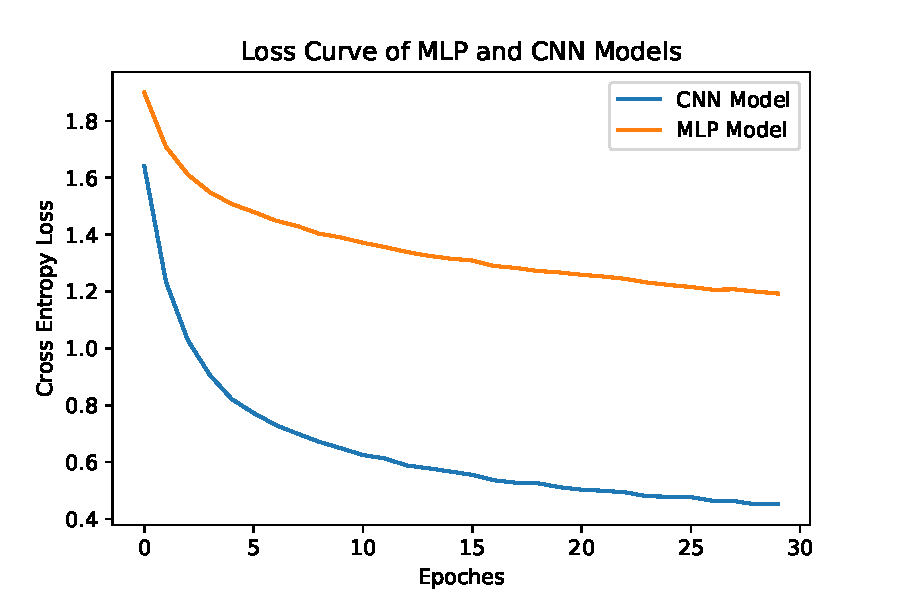
\includegraphics[width=0.8\textwidth]{Loss_Curve_MLP_CNN}
	\caption{Training loss of MLP and CNN model over 30 epochs}
	\label{fig:loss_curve_mlp_cnn}
\end{figure*}

\subsection*{Comparing MLP and CNN model}
CNN model outperform MLP model in terms of test accuracy. But MLP model seems more efficient to compute. A possible reason is CNN's kernel sturcture can better capture the feature of images (i.e., edge features)

\subsection*{Model with/without Avtication Function}
In this section, I did an experiment on training MLP, CNN models with and without non-linear activation functions. The loss curve are plotted as following (in Figure \ref{fig:activation}):

\begin{figure}[h]
  \centering
  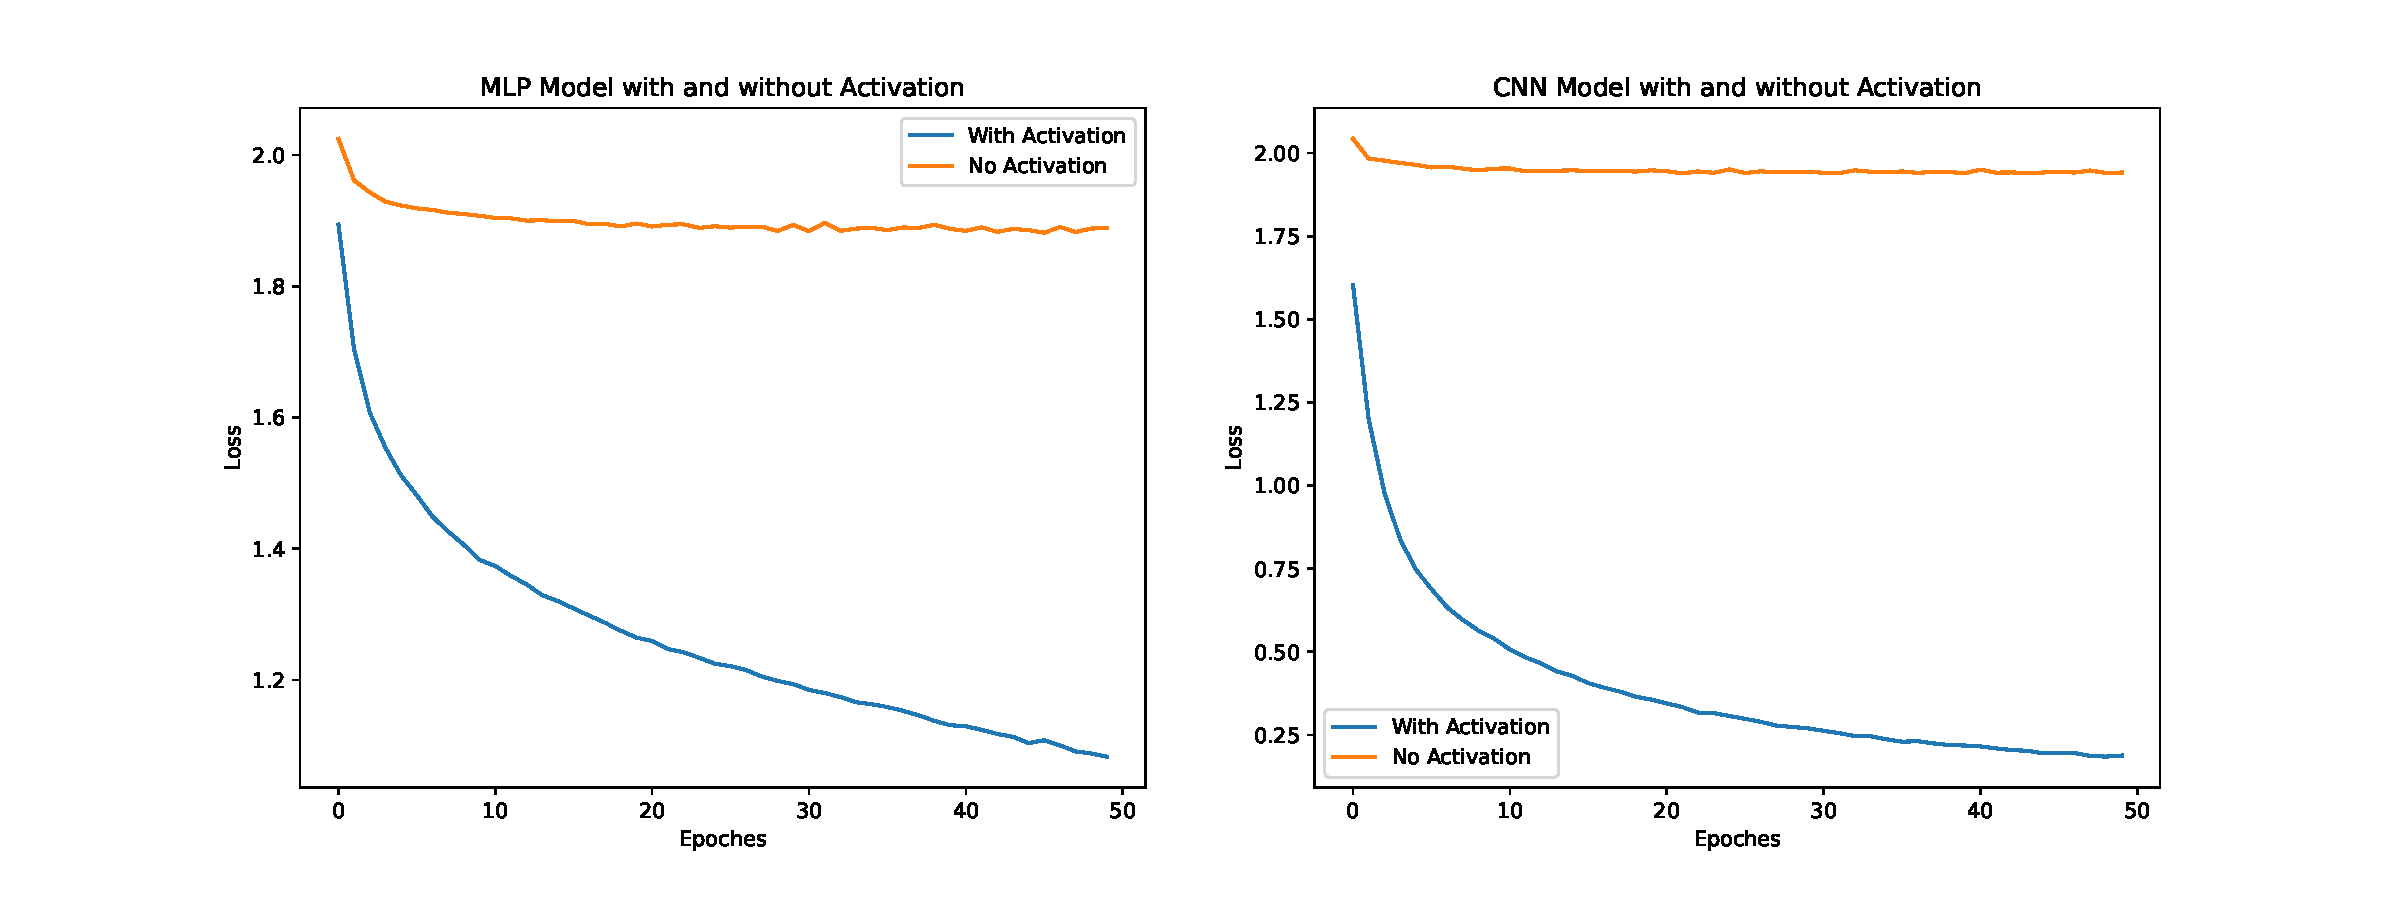
\includegraphics[width=\textwidth]{Activation_NO_Activation.pdf}
  \caption[]{Training loss of MLP and CNN model with/without non-linear activation function}
  \label{fig:activation}
\end{figure}

From the figure, we can know that without activation function, the loss stop to decrease in a early stage during training. The final accuracy without activation function cannot really catch up with the performance with a normal MLP/CNN model.

This finding probably echos the effect of non-linear activation function: combining multiple hyperplanes to construct a non-linear hypothesis.

\end{document}
